% \newpage
\section{Discussion}
\label{sec: discussion}

\autoref{thm: convergence mcopi uniform} showed that initial-visit MC-O-PI converges almost surely to $\qopt$ 
% for a contractive MDP 
when updates are uniform over the actions in each state.
% or, equivalently, when they are uniform over the deterministic policies.
% 
% provided
% that the learning rates satisfy the Robbins--Monro conditions and the comparability property,
% % the update functions are initial-visit,
% that the sampling distributions satisfy strict exploring starts,
% and that the resulting update distributions are uniform over all actions in each state.
% 
This section explores the implications of this result.
We first explain that the uniformity condition effectively requires using initial-visit updates, which does not necessarily slow down convergence compared to first-visit updates.
We then describe how to generalise this result to optimistic policy-iteration algorithms with temporal-difference updates, or when the estimate $q_k$ is stored approximately at every step.
Finally, we argue that some conditions can likely be relaxed because they are not essential for the underlying improvement process.


% as the condition for uniform updates forces the use of initial-visit method
% Even if initial-visits is less data-efficient than first-visits, this does not mean that solutions converge slower to the optimal policy.


%%%%%%%%%%%%%%%%%%%%%%%%%%%%%%%%%%%%%%%%%%%%%%%%%%%%%%%%%%%%%%%%%%%
%%%%%%%%%%%%%%%%%%%%%%%%%%%%%%%%%%%%%%%%%%%%%%%%%%%%%%%%%%%%%%%%%%%
\subsection{Uniform updates effectively force initial-visits}


When the underlying MDP is unknown, using first- or every-visit updates causes the update distribution $\mu_k$ to depend on the unknown transition dynamics induced by policy $\pi_k$.
Therefore, requiring uniform update distributions effectively forces the use of initial-visit updates,
% because we cannot determine how the initial sampling distribution $\sigma_k$ will propagate through the MDP under policy $\pi_k$. 
because by updating only the initial state-action pair of each episode, we ensure $\mu_k$ equals $\sigma_k$ and thus retain control.

This control comes at the cost of data efficiency: the initial-visit method discards within-episode transitions that the first-visit method would reuse. However, more updates per episode do not automatically translate into faster policy convergence.
The extra updates induce a bias in the update distribution that can generate sliding modes in the action-value estimates $(q_k)_{k \ge 0}$ and thereby slow down the convergence of the policy sequence $(\pi_k)_{k \ge 0}$. Ultimately, it is the convergence speed of this policy sequence that truly matters for identifying the optimal behaviour of the MDP.

% describe MDP
To illustrate this, consider the MDP in \autoref{fig: experiment smallest MDP for iv vs fv} with a discount factor $\discount = 0.5$. Action \textit{left} yields a reward of one and \textit{right} yields a reward of zero.
% The best policy $\best{\pol}$ follows the \textit{left} action, whereas the worst policy $\worst{\pol}$ follows the \textit{right} action.
% describe learning algorithm
Under a uniform sampling distribution $\sigma_k$, the intial-visit method updates exactly one state-action pair per episode, whereas the first-visit method updates on average $1.5$ pairs.
With a learning rate $\alpha_k = 1/(k+100)$, the first-visit method also benefits from larger effective steps because it updates state-action pairs more frequently.
% Despite this numerical advantage, experiments show that IV can convergence to $\pi^*$ sooner.


Despite this apparent advantage, the initial-visit method is more stable than first-visit when MC-O-PI is initialised above $\qopt$.
Namely, initial-visit solutions follow straight lines that always point towards better policies.
In contrast, first-visit solutions exhibit a sliding mode that causes high-frequency oscillations in the policy sequence and traps $q_k$ near the boundary for longer.
As a result, first-visit can take longer to settle on the optimal policy.
For instance, when averaging over 1000 solutions starting in $q'$, first-visit ones require on average 43 updates to settle on $\pi_*$, whereas initial-visit ones always remain in $\region(\best{\pi})$.
When starting in $q$, the solutions take 68 and 70 updates to settle on $\pi_*$.


Overall, this experiment illustrates that the initial-visit method can be practical in real-world applications. 
By avoiding sliding modes, it sometimes converges to the optimal policy $\best{\pi}$ as fast as, or faster than, the first-visit method despite fewer updates and smaller effective learning rates.
Besides, the initial-visit method is more reliable for early stopping. Namely, if training stops early, the last greedy policy of an initial-visit solution is typically the best policy encountered so far, whereas the first-visit solution may be oscillating across a decision boundary, making it unclear which policy is best.

% Namely, since the policy sequence transitions almost smoothly instead of oscillating, terminating the algorithm prematurely yields a policy that reliably reflects the best policy found so far. In contrast, stopping a first-visit trajectory early risks catching it across a decision boundary, leaving it unclear which policy is actually best.


% since the initial-visit method experiences no sliding modes, 
% it can converge as fast as, or faster than, the first-visit method to $\best{\pi}$, even with fewer updates and smaller effective learning rates. Furthermore, the absence of sliding mode makes
% , the current policy is a more reliable “best-so-far” policy. So if training stops early, the IV iterate typically reflects the best policy reached so far, while FV may still oscillate across the decision boundary, making it unclear which policy is best.

% this problem is not conthrived
% - happens when overestimate the action values (a priori dont know them)
% - dont know how strong the greedy bias with FV is, this is the region with potential sliding modes

% if we use learning rate $1/n(s,a)$
% actually helps FV because learning rate decreases the greedy bias


\begin{figure}[t!]
    \centering
    \begin{subfigure}[b]{\textwidth}
        \centering
        % \begin{tikzpicture}[
        %     scale=1, auto, node distance=2cm, 
        %     every edge/.style={draw, <-, font=\small},
        %     state/.style={circle, fill=mylightgrey, draw=black, text=black}
        % ]
        %     % Nodes
        %     \node[state] (s1) at (0,0) {$s$};
        %     % Edges
        %     \path[->]
        %         (s1) edge[out=160, in=200, loop, looseness=8, draw=black] node[pos=0.5, left, text=black] {\textcolor{mygrey}{$\best{\pi}(s) :=$} 1} (s1)
        %         (s1) edge[out=20, in=340, loop, looseness=8, draw=black] node[pos=0.5, right, text=black] {0 \textcolor{mygrey}{$=: \worst{\pi}(s)$}} (s1) ;
        %         % (s1) edge[out=145, in=215, loop, looseness=7] 
        %         %     node[pos=0.5, right] {$\best{a}$} 
        %         %     node[pos=0.5, left] {1} 
        %         % (s1)
        %         % (s1) edge[out=35, in=325, loop, looseness=7] 
        %         %     node[pos=0.5, left] {$\worst{a}$} 
        %         %     node[pos=0.5, right] {0} 
        %         % (s1);
        % \end{tikzpicture}
        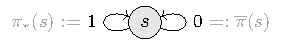
\includegraphics[width=0.35\linewidth]{figures/mdp.pdf}
        \caption{MDP}
        \label{fig: experiment smallest MDP for iv vs fv}
    \end{subfigure}%
    \\
    \vspace{0.5cm}
    % --- Subfigure 1: Streamlines ---
    \begin{subfigure}[b]{0.48\textwidth}
        % \begin{tikzpicture}
        %     \begin{axis}[
        %         width=\linewidth,
        %         % title={Initial-visit solutions},
        %         xlabel={$q(s, \pi_*(s))$},
        %         ylabel={$q(s, \overline \pi(s))$},
        %         tick label style={font=\small},
        %         label style={font=\small},
        %         xmin=0, xmax=5,
        %         ymin=-0.5, ymax=4.5,
        %         % grid=off,
        %         axis equal image,
        %         unbounded coords=jump, % This handles the NaN values in your CSV
        %         xtick={1, 2,4},
        %         % xticklabels={1, $\frac{1}{1-\gamma}$, 4},
        %         ytick={0, 1,4}
        %     ]

        %         \addplot [black, thin, dotted, domain=-0.5:5, samples=2] {x};
                
        %         % 1. Plot the streamlines from CSV
        %         \addplot[mygrey, thin, forget plot] table [col sep=comma, x index=0, y index=1] {figures/streamlines-iv.csv};

        %         % 2. Plot the simulation trajectory
        %         \addplot[CambridgeCoreBlue, thick] table [col sep=comma, x index=0, y index=1] {figures/simulation-iv-above.csv};

        %         \addplot[CambridgeCoreBlue, thick] table [col sep=comma, x index=0, y index=1] {figures/simulation-iv-below.csv};
                
        %         % 3. Mark Attractors (x1 and x2 based on your gamma=0.5)
        %         \node[label={right:$q_{\pi_*}$}, circle, fill, inner sep=1.5pt] at (axis cs:2, 1) {};
                
        %         \node[label={right:$q_{\overline \pi}$}, circle, fill, inner sep=1.5pt] at (axis cs:1,0) {};
                
        %         % 4. Start Points with Labels
        %         % Point A: Using your x0 = [3.75, 4]
        %         \node[label={left:$q$}, circle, fill, inner sep=1.5pt, CambridgeCoreBlue] at (axis cs:3.75, 4) {};
                
        %         % Point B: Placeholder (Update coordinates as needed)
        %         \node[label={below:$q'$}, circle, fill, inner sep=1.5pt, CambridgeCoreBlue] at (axis cs:4, 3.75) {};
        %     \end{axis}
        % \end{tikzpicture}
        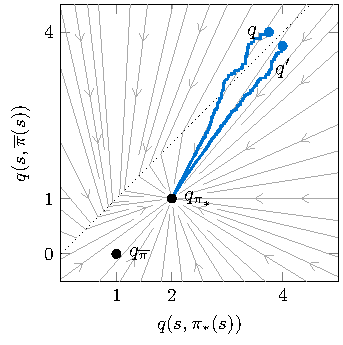
\includegraphics[width=0.8\linewidth]{figures/iv-sol.pdf}
        \caption{Initial-visit solutions}
        \label{fig: iv versus fv simulations IV}
    \end{subfigure}
    \hfill
    % --- Subfigure 2: Placeholder or Second Simulation ---
    \begin{subfigure}[b]{0.48\textwidth}
        % \begin{tikzpicture}
        %     \begin{axis}[
        %         width=\linewidth,
        %         % title={First-visit solutions},
        %         xlabel={$q(s, \pi_*(s))$},
        %         ylabel={$q(s, \overline \pi(s))$},
        %         tick label style={font=\small},
        %         label style={font=\small},
        %         xmin=0, xmax=5,
        %         ymin=-0.5, ymax=4.5,
        %         % grid=off,
        %         axis equal image,
        %         unbounded coords=jump, % This handles the NaN values in your CSV
        %         xtick={1, 2,4},
        %         % xticklabels={1, $\frac{1}{1-\gamma}$, 4},
        %         ytick={0, 1,4}
        %     ]

        %         \addplot [black, thin, dotted, domain=-0.5:5, samples=2] {x};
                
        %         % 1. Plot the streamlines from CSV
        %         \addplot[mygrey, thin, forget plot] table [col sep=comma, x index=0, y index=1] {figures/streamlines-fv.csv};

        %         % 2. Plot the simulation trajectory
        %         \addplot[CambridgeCoreBlue, thick] table [col sep=comma, x index=0, y index=1] {figures/simulation-fv-above.csv};

        %         \addplot[CambridgeCoreBlue, thick] table [col sep=comma, x index=0, y index=1] {figures/simulation-fv-below.csv};
                
        %         % 3. Mark Attractors (x1 and x2 based on your gamma=0.5)
        %         \node[label={right:$q_{\pi_*}$}, circle, fill, inner sep=1.5pt] at (axis cs:2, 1) {};
                
        %         \node[label={right:$q_{\overline \pi}$}, circle, fill, inner sep=1.5pt] at (axis cs:1,0) {};
                
        %         % 4. Start Points with Labels
        %         % Point A: Using your x0 = [3.75, 4]
        %         \node[label={left:$q$}, circle, fill, inner sep=1.5pt, CambridgeCoreBlue] at (axis cs:3.75, 4) {};
                
        %         % Point B: Placeholder (Update coordinates as needed)
        %         \node[label={below:$q'$}, circle, fill, inner sep=1.5pt, CambridgeCoreBlue] at (axis cs:4, 3.75) {};
        %     \end{axis}
        % \end{tikzpicture}
        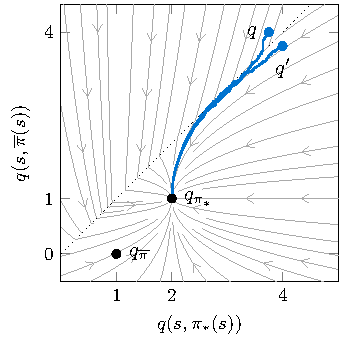
\includegraphics[width=0.8\linewidth]{figures/fv-sol.pdf}
        \caption{First-visit solutions}
        \label{fig: iv versus fv simulations FV}
    \end{subfigure}
    \caption{By avoiding sliding modes, initial-visit solutions sometimes converge to the optimal policy $\best{\pi}$ faster than first-visit solutions despite fewer updates and smaller effective learning rates. The blue lines are MC-O-PI solutions starting in $q$ or $q'$, whereas the grey lines indicate the mean-field flow.}
    \label{fig: iv versus fv simulations}
\end{figure}



%%%%%%%%%%%%%%%%%%%%%%%%%%%%%%%%%%%%%%%%%%%%%%%%%%%%%%%%%%%%%%%%%%%
%%%%%%%%%%%%%%%%%%%%%%%%%%%%%%%%%%%%%%%%%%%%%%%%%%%%%%%%%%%%%%%%%%%
%\subsection{Guaranteeing convergence with non-uniform updates}

% The practical takeaway from this paper is simple: if MC-O-PI seems trapped in a suboptimal limit set (on a boundary or in a cycle), 
% then using initial-visit updates
% with uniform sampling distributions over the actions in each state
% guarantees that the algorithm eventually converges to the optimal policy and its action values
% while avoiding slow sliding modes.

% In order to turn non-uniform update distributions into uniform effective updates, \cite{Tsitsiklis2002OnIteration} suggests making the learning rates inversely proportional to the update distribution.
% In a model-free setting, this strategy only applies if the update distributions are generated with the initial-visit method.
% This is because the first-visit method causes the update distributions to depend on the transition dynamics induced by the currently greedy policy on the MDP.
% Since the greedy policy changes at every step and the structure of the MDP is unknown,
% we must assume that first-visit update distributions change at every step.
% Cancelling out these changing, non-uniform distributions thus requires knowing the induced transition dynamics, which are unpredictable if the MDP is unknown.

% Nonetheless, consider non-uniform, initial-visit update distributions $(\mu_k)_{k \ge 0}$, which essentially equal the sampling distributions $(\sigma_k)_{k \ge 0}$.
% For any scalar sequence $(\lambda_k)_{k \ge 0}$ that satisfies the Robbins--Monro conditions,
% if the $k^\nth$ episode starts in $(s_0, a_0)$, then setting
% \[
%     \alpha_k = \frac{\lambda_k}{\sigma_k(s_0, a_0)} , 
% \]
% guarantees that the effective learning rates in MC-O-PI's difference inclusion are uniform because $\alpha_k \, \mu_k(s_0, a_0) = \lambda_k$.
% However, this approach is impractical because it requires knowing the sampling probability for each state-action pair at every step,
% or, if these probabilities are constant over time, tracking the number of updates of each state-action pair \citep[p.~66]{Tsitsiklis2002OnIteration}.


% Tsitsiklis notes that MC-O-PI's asymptotic behaviour depends on the asymptotic behaviour of the effective learning rates $(\lrate_k \update_k)$, not on either component alone.
% For instance, if the update distributions are non-uniform but constant, say $\update_k = \update$ for all $k$, and the learning rates take the form $\lrate_k(s,a) = 1/n_k(s,a)$, where $n_k(s,a)$ denotes the number of updates of $(s,a)$ in the first $k$ steps,
% then $\lrate_k \update_k$ converges to $1/k$ because for each state-action pair $n_k(s,a)$ tends to $k \update(s,a)$. As a result, updates are eventually uniform. So \autoref{thm: convergence mcopi uniform} still applies.


% In contrast, we showed that global convergence only requires uniform updates over all actions in each state.
% Using the decomposition
% \[
% \sigma_k(s,a) = \sigma^{\sset}_k(s) \, \sigma^{\aset}_k(a \mid s)
% \]
% where $\sigma^{\sset}$ represents the sampling distribution over the state space,
% and $\sigma^{\aset}$ is the distribution over the action space of each state,
% it is thus sufficient to choose learning rates as
% \[
%     \alpha_k = \frac{\lambda_k}{\sigma^{\aset}_k(a_0 \mid s_0)}.
% \]
% This is more practical because it only assumes knowing the sampling probability of the initial action $a_0$ relative to the other actions of the initial state $s_0$, rather than all other state-action pairs.
% In other words, we can obtain global convergence 
% by turning non-uniform update distributions 
% into uniform effective updates even if the initial state is sampled from an unknown distribution, provided the distribution of the initial action in that state is known. This occurs in practice, for instance, when selecting the initial action using an $\varepsilon$-greedy strategy.


% A concrete example of a non-uniform update distribution arises when biasing updates towards the greedy actions to \textit{exploit} the policy that is currently believed to be optimal.
% However, by unevenly updating actions, this approach causes non-greedy actions to evolve very slowly and potentially leads to the sliding modes depicted in \autoref{fig: iv versus fv simulations}.
% Therefore, if we additionally scale down the learning rates for the greedy actions in proportion to their increased update probability (so that the product $\alpha_k(s,a)\,\mu_k(s,a)$ does not depend on $a$),
% then updates are effectively uniform over the actions of each state, and global convergence is guaranteed.
% Notably, this adjustment does not violate the comparability property (\autoref{asp: additional conditions on learning rate}) required by \autoref{thm: convergence mcopi uniform}. Although learning rates may fail global comparability across the entire process, the proof only uses the comparability property between transitions, which matches the intervals in which the greedy actions remain the same.
% An additional benefit of making the learning rates inversely proportional to the update distribution is that this reduces the variance of the estimate $q_k$ for greedy actions, which means the solution remains closer to the well-behaved mean-field solution along that dimension.
% On the other hand, the larger learning rates for non-greedy actions compensate for their infrequent updates but at the cost of slightly increased variance.
% Ultimately, this learning rate adjustment 
% % removes the convergence difficulties seen with purely greedy updates (such as slow learning for non-greedy actions, or sliding modes), keeps all trajectories well-behaved, and 
% ensures that all action values converge at similar rates along approximately straight trajectories towards the optimum.


% %%%%%%%%%%%%%%%%%%%%%%%%%%%%%%%%%%%%%%%%%%%%%%%%%%%%%%%%%%%%%%%%%%%
% %%%%%%%%%%%%%%%%%%%%%%%%%%%%%%%%%%%%%%%%%%%%%%%%%%%%%%%%%%%%%%%%%%%
% \subsection{Importance of noise}
% \label{sec: discussion noise}


% general comment to anybody studying
% switching linear system

% stochastic difference equation

% proof is not an iff

% stochastic solutions can lock into the region of a policy thanks to noise even when the mean-field




%%%%%%%%%%%%%%%%%%%%%%%%%%%%%%%%%%%%%%%%%%%%%%%%%%%%%%%%%%%%%%%%%%%
%%%%%%%%%%%%%%%%%%%%%%%%%%%%%%%%%%%%%%%%%%%%%%%%%%%%%%%%%%%%%%%%%%%
\subsection{Mean-field analysis with temporal difference updates}
\label{sec: discussion temporal difference}

The growth and lock-in events only require unbiased noise with eventually bounded variance, and the seed event is a simple finite-horizon process to guarantee that solutions can overcome the decreasing margin.
These events should therefore also make it possible to derive global convergence of optimistic policy-iteration algorithms with temporal-difference updates from their mean-field dynamics.
The additional difficulty would be to understand how the position of the estimate $q$ and the depth $n$ of the episode simulations affect the target $T_{\pi}^n q$, where $\pi \in P(q)$ and $T_\pi$ is the Bellman operator associated with policy $\pi$.


%%%%%%%%%%%%%%%%%%%%%%%%%%%%%%%%%%%%%%%%%%%%%%%%%%%%%%%%%%%%%%%%%%%
%%%%%%%%%%%%%%%%%%%%%%%%%%%%%%%%%%%%%%%%%%%%%%%%%%%%%%%%%%%%%%%%%%%
\subsection{MC-O-PI with function approximation}
\label{sec: discussion function approximation}

\autoref{thm: convergence mcopi uniform} applies specifically to \textit{tabular} MC-O-PI, where the estimate $q_k$ can be stored exactly.
In practical applications, however, the estimate is approximated, for instance using a neural network.
In this setting, the error between the observed return and the current estimate is then used to update the parameters of the approximation.
% for instance using gradient descent.

With a sufficiently rich approximation method,
the approximation error should only contribute a finite perturbation to the MC-O-PI difference inclusion.
This suggests that \autoref{thm: convergence mcopi uniform}
can be generalised with function approximation using the results in \citep[Section~4.3.3]{Bertsekas1996Neuro-DynamicProgramming} or \citep[Section~5.2]{Kushner2003StochasticApplications}.
%Furthermore, integrating a normalisation trick as in \autoref{sec: normalisation trick} into Monte Carlo Tree Search might accelerate AlphaZero's or MuZero's learning process by mitigating slow sliding modes.

% Finally, \citet{Wagner2013OptimisticResult} shows that policy gradient methods
% % which underlie recent breakthroughs in natural language processing and robotics \citep{Schulman2017ProximalAlgorithms}, 
% can be interpreted as optimistic policy iteration algorithms with function approximation. Extending our results to this setting might
% thus improve the efficiency and performance of these essential methods.


Finally, recent breakthroughs in natural language processing and robotics~\citep{Schulman2017ProximalAlgorithms} rely on policy gradient methods.
\citet{Wagner2013OptimisticResult} shows that some of these methods can be interpreted as optimistic policy iteration algorithms with function approximation.
Extending our results to this setting might thus improve the efficiency and performance of these essential methods.


% \textcolor{red}{still necessary?}

% Applying the method of \autoref{sec: results} when update distributions are uniform over all state-action pairs 
% reveals a Lyapunov interpretation of Tsitsiklis' framework.
% Namely, consider the potential function that measures the one-sided Bellman residual
% \begin{align}
%     \tilde V(q) = \frac{1}{2} \|(q-\B q)_+\|_2^2 .
% \end{align}
% Its gradient is
% \begin{align}
%     \nabla \tilde V (q) = (I - \discount P_\pi )^\top (q-\B q)_+
% \end{align}
% where $\pi$ is any deterministic policy that is greedy with respect to $q$.
% Computing the inner product with the mean-field update of MC-O-PI yields
% \begin{align*}
%     \langle \nabla \tilde V(q) , q_\pi - q \rangle
%     &= \langle (I - \discount P_\pi )^\top (q-\B q)_+ , (I - \discount P_\pi )^{-1} (\B q - q) \rangle
%     \\
%     &= \langle (q-\B q)_+ , (\B q - q) \rangle
%     \\
%     &= - \|(q - \B q)_+\|_2^2
%     \\
%     &= - 2 \tilde V(q)
% \end{align*}
% Thus, when updates are uniform over all state-action pairs, the mean-field update $(q_\pi - q)$ is a strict descent direction for the potential $\tilde V$.
% This geometric insight corresponds to the decrease in inequality \eqref{eq: q-Bq decreases} that is essential to Tsitsiklis' proof.
% % That proof thus exploits the tension between the fact that every limit point is upper and lower bounded by the best and worst action values of the corresponding greedy policies (\autoref{thm: bounded limit sets})
% % and that such point has a strictly positive one-sided Bellman residual (\autoref{thm: bellman residual has positive component}).
% The proof in \autoref{sec: results} builds on this insight. 
% Unlike Tsitsiklis' method, our proof does not rely on the commutativity of the transition matrix $P_\pi$ and the update distribution $\mu$. The trade-off is that we must instead constrain the variation of the update distribution to ensure that the local descent property is preserved.
% Yet, as discussed earlier, we expect that this conditions can be relaxed.

% We note that Tsitsiklis extends his proof to optimistic policy iteration with temporal difference returns, i.e. where the target $q_\pi$ is replaced by a geometrically weighted sum of multi-step returns (TD($\lambda$)).
% This introduces an additional error term in the descent inequality \eqref{eq: q-Bq decreases}. Given the structural similarities, we conjecture that the framework of \autoref{sec: results} can be similarly extended. Future work could apply our method to TD-O-PI, where an analogous summable error term would likely appear in the critical inequality \eqref{eq: V goes to infinity}, potentially establishing convergence for TD control under our broader class of update distributions.


% Tsitsiklis proof also works with temporal difference optimistic policy iteration
% $n$-step TD-O-PI is when updates are
% \begin{align}
%     q_{k+1} \in 
%     \{
%     q+k + \lrate_k \update_k (\B_\pi^n q_k - q_k + w_k)
%     \}
% \end{align}
% with the appropriate definition of stochastic perturbations.
% so $n=1$ is q learning whereas $n=\infty$ is MC-O-PI

% not sure whether the argument is exactly symmetrical ...
% the argument in \autoref{sec: results} is symmetrical. All that matters is that $\bqar q \neq \B \bar q$. either focus on state-action pairs where $[\bar q(s,a) - \B \bar q](s,a)>0$ and then use the definition of $g_\pi$ and $V$ as above. or focus on states where $[\bar q(s,a) - \B \bar q](s,a) < 0$ and then use the definition of $g_\pi \coloneqq \mu^{-1} (I - \discount P_\pi^\top)(\B \bar q - q)_+$ and $V(q) \coloneqq \min_\pi \langle g_\pi, q - \bar q \rangle$ and show that $q_k \to \bar q$ drives V to $- \infty$.


%%%%%%%%%%%%%%%%%%%%%%%%%%%%%%%%%%%%%%%%%%%%%%%%%%%%%%%%%%%%%%%%%%%
%%%%%%%%%%%%%%%%%%%%%%%%%%%%%%%%%%%%%%%%%%%%%%%%%%%%%%%%%%%%%%%%%%%
\subsection{Relaxing conditions}
\label{sec: relaxing conditions}

% - assumption that limit set reduces to a point => this is assumption on solution, not on algorithm

% relax
% - policy samping => update only policy in state that changed, then dont even need event $\mathcal E^t_k$
% - essentially just need comparison prop of leanring rates to ensure reach fixed distance into a region, if can show other way, then just need Borkar lock in, i.e. \autoref{thm: event noise remains small}

% Technically, 
The proof of \autoref{thm: convergence mcopi uniform}
requires a uniform lower-bound on the distribution of the greedy policy at each step, strict exploring starts and non-increasing, comparable learning rates.
However, these conditions are artefacts of the framework of the proof rather than necessary conditions for the underlying policy improvement process.


For instance, the global seed event updates only one state-action pair per step. 
% Yet the greedy policy can be updated for all states at every step.
Yet since the greedy policy is updated for all states at every step, it can change in any state with ties.
Sampling the greedy policy, as described in \eqref{eq:greedy-pol-tie-breaking}, 
therefore prevents
adversarial tie-breaking from always worsening the policy by choosing $\pi_{k+1}(s)=a$
whenever
% if after the $k^{\text{th}}$ update,
$q_{k+1}(s,\pi_k(s)) = q_{k+1}(s,a)$ but $q_{\pi_k}(s,\pi_k(s)) > q_{\pi_k}(s,a)$.
% the gap of a pair in $\mathcal B_\pi$ is zero after an update,
% , and thereby invalidate \autoref{thm: fixed prob that bad actions dont become greedy}.
% (see the discussion from equation \eqref{eq: joint intermediate event} onwards)
Such ties are rare in practice;
% except if the algorithm is initialised in one.
moreover, updating the greedy policy for all states at every step is inefficient.
A more practical method under initial-visit updates is to only recompute the policy in the state that was updated at step $k$.
%by comparing $q_{k+1}(s, \pi_{k}(s))$ with $q_{k+1}(s, a)$ where $u_{k}(s,a) = 1$.
This method simplifies the proof of \autoref{thm: convergence mcopi uniform} as the global tie-breaking event \eqref{eq: def global tie event} is no longer necessary,
given that ties are broken once, right after the transition, 
and remain unchanged until the corresponding seed event makes the policy-worsening action non-greedy.
% until the pair is updated by the corresponding seed event,
% which can only increase the gap and hence break the tie in favour of the currently greedy action.


Further, the strict exploring starts, and the non-increasing and comparability conditions on the learning rates ensure that the stochastic perturbations cannot persistently offset the mean-field dynamics.
Specifically, they guarantee through the seed and growth events
% \eqref{eq: def global seed event}--\eqref{eq: def global grow event}
that
for every policy $\pi \in \mathcal P$,
the stochastic perturbations cannot force the sequence
$(q_k(s,\pi(s)) - q_k(s,a))_{k \ge 0}$ to converge to zero 
on the subsequence of times $\{k \ge 0 : \pi_k = \pi\}$
if $q_{\pi}(s,\pi(s)) > q_{\pi}(s,a)$.
However, given the Robbins--Monro learning rates and the martingale difference noise sequence,
the accumulated stochastic perturbations form a converging martingale sequence, and hence $\lim_{K \to \infty} \sum_{k \ge K} \alpha_k w_k = 0$.
As a result, we expect that there exists another way to establish that the perturbations do not contain enough energy to consistently counteract the mean-field dynamics.
% , likely using an equivalent of the Robbins-Siegmund Theorem.

% If can prove another way, then can use the lock-in phenomenon and the combined stability-ODE method described in Section \ref{sec: limitations of existing methods}.

% %\textcolor{red}{is all this necessary? Could just skip to stating the minimal requirements}
Since the monotone improvement that drives convergence when updates are uniform does not hinge on these conditions, we expect that they can be relaxed.
Nevertheless, some constraints on the update distributions will always remain necessary as they effectively scale the learning rates in the MC-O-PI difference inclusion \eqref{eq: mcopi not yet sri}.
% leading to different learning rates for different state-action pairs.
Namely, convergence to a fixed point requires Robbins–Monro–like conditions on the products $(\lrate_k \update_k)$, not on $(\lrate_k)$ alone.

% To make sure that the effective learning rates for each pair are large enough to avoid premature convergence due to Zeno-like behaviour while gradually decreasing to zero so that noise cannot prevent convergence, it is that the Robbins--Monro conditions will have to be satisfied on the product $(\lrate_k \update_k)$ rather than on the learning rates alone.

To see why the Robbins--Monro conditions must be adjusted, fix a policy $\pi$ and consider the system
\begin{align}
\label{eq: single system}
    q_{k+1}
    &= q_k + \lrate_k \update_k (q_\pi - q_k) + \lrate_k w_k .
\end{align}
Unrolling over $n$ steps yields
\begin{align*}
    q_{k+n}
    = \left( \prod_{i=k}^{k+n-1} (\mathsf{I} -\lrate_i \update_i) \right) q_k 
    + \left( \mathsf{I} - \prod_{i=k}^{k+n-1} (\mathsf{I} -\lrate_i \update_i) \right) q_\pi
    % \\
    + \sum_{j=k}^{k+n-1} \prod_{i=j+1}^{k+n-1} (\mathsf{I} -\lrate_i \update_i) \lrate_j w_j .
\end{align*}
For $q_{k+n}$ to converge to $q_\pi$ as $n$ grows to $\infty$, three conditions must be satisfied for every state $s \in \sset$ and action $a \in \aset(s)$.
First,
\begin{align}
\label{eq: condition infinite visits}
    \sum_{k=0}^{\infty} \update_k(s,a) = \infty ,
    % \qquad \forall \, s \in \sset, \forall \, a \in \aset(s) .
\end{align}
so that the state-action pair is updated infinitely often.
% Therefore, for every state-action pair $(s,a)$, the update distributions $(\update_k)$ must satisfy
Second, 
\begin{align}
    \label{eq: condition infinite effective learning rate}
    \sum_{k=0}^{\infty} \lrate_k \update_k(s,a) = \infty ,
    % \qquad \forall \, s \in \sset, \forall \, a \in \aset(s) .
\end{align}
so that the product $\prod_{i=k}^{k+n-1} (1 - \lrate_i \update_i(s,a))$ decays to zero for increasing $n$.
Finally,
\begin{align}
    \label{eq: summable learning rates outside def}
    \sum_{k=0}^\infty \lrate_k^2 < \infty ,
\end{align}
to ensure the accumulated stochastic perturbations vanish.

% If we imposed $\sum_k \lrate_k^2 \update_k^2 < \infty$ instead, we could choose $\lrate_k = \update_k(s,a) = 1/\sqrt{k}$ for each state-action pair, still satisfy conditions \eqref{eq: condition infinite visits} and \eqref{eq: condition infinite effective learning rate}. However, the noise term in \eqref{eq: single system unrolled} would become
% \begin{align}
%     \sum_{j=k}^{k+n-1} \prod_{i=j+1}^{k+n-1} (1-\frac{1}{i}) \frac{1}{\sqrt{j}} \xi_j
%     &= \sum_{j=k}^{k+n-1} \frac{j}{k+n+1} \frac{1}{\sqrt{j}} \xi_j
%     \\
%     &= \frac{1}{k+n+1} \sum_{j=k}^{k+n-1} \sqrt{j} \xi_j
%     \\
%     &\eqqcolon N_{k,n}
% \end{align}
% We see that
% \begin{align}
%     \E[N_{k,n}^2] = \E \Bigg[ \Big( \frac{1}{k+n+1} \sum_{j=k}^{k+n-1} \sqrt{j} \xi_j \Big)^2 \Bigg]
% \end{align}
% Since the cross terms vanish in expectation, 
% and as a result, $q_k$ would not converge to $q_\pi$
% 
% since $\sum_k \lrate_k^2 = \infty$, the noise would not be almost surely bounded. In other words, the noise alone would be able to pull solution arbitrarily far from $q_\pi$ infinitely often, thereby preventing convergence.
% 
Note that \eqref{eq: condition infinite visits} does not automatically imply \eqref{eq: condition infinite effective learning rate}.
For instance, under \eqref{eq: condition infinite visits} and the Robbins--Monro conditions on the learning rates $(\lrate_k)$, we could choose $\lrate_k = \update_k(s,a) = 1/k$. System \eqref{eq: single system} would then converge prematurely due to Zeno-like behaviour because the products $\prod_{i=k}^{k+n-1} (1-\lrate_i \update_i(s,a))$ would not decay to 0.


Altogether, the minimal requirements on the learning rates and the update distributions are
% for every state $s \in \sset$ and action $a \in \aset(s)$
\begin{align}
    \label{eq: xtn robbins-monro first}
    &\sum_{k =0}^\infty \lrate_k \update_k(s,a) = \infty 
    \qquad \forall \, s \in \sset, \forall \, a \in \aset(s) ,
    \\
    \label{eq: xtn robbins-monro second}
    &\sum_{k =0}^\infty \lrate_k^2 < \infty ,
\end{align}
because \eqref{eq: xtn robbins-monro second} implies that, eventually, $\alpha_k \mu_k < \mu_k$, and \eqref{eq: xtn robbins-monro first} then lower bounds \eqref{eq: condition infinite visits}.
We expect the results from Section~\ref{sec: results} to extend under these milder conditions.


% The update distributions $(\update_k)$ may depend on the policies $(\pol_k)$ and thus be unknown before running MC-O-PI.
% Nevertheless, it is possible to select learning rates, start distributions and update functions so that the above conditions hold.
% For initial-visit updates, it suffices to verify that the sequences $(\lrate_k)$ and $(\start_k)$ satisfy these conditions.
% If they do, the conditions remain valid under first-visit updates, regardless of the policies $(\pol_k)$.


% Furthermore, ...
% only the values in the limit matter for asymptotic analysis

% e.g. update distribution
% e.g. policy
% the GLIE conditions (\autoref{def: glie}) require that in the limit the policy $\pol$ is greedy with respect to the estimate $q$ so that solutions stop moving once they reach the optimal policy $\best{\pol}$ and action values $\qopt$.
% Since we study the asymptotic behaviour of MC-O-PI, we will assume that the policy is greedy at every step.

% Tsitsiklis notes that MC-O-PI's asymptotic behaviour depends on the asymptotic behaviour of the effective learning rates $(\lrate_k \update_k)$, not on either component alone.
% For instance, if the update distributions are nonuniform but constant, say $\update_k = \update$ for all $k$, and the learning rates take the form $\lrate_k(s,a) = 1/n_k(s,a)$, where $n_k(s,a)$ denotes the number of updates of $(s,a)$ in the first $k$ steps,
% then $\lrate_k \update_k$ converges to $1/k$ because for each state-action pair $n_k(s,a)$ tends to $k \update(s,a)$. As a result, \autoref{thm: c(q) goes to zero} still applies.




%%%%%%%%%%%%%%%%%%%%%%%%%%%%%%%%%%%%%%%%%%%%%%%%%%%%%%%%%%%%%%%%%%%
%%%%%%%%%%%%%%%%%%%%%%%%%%%%%%%%%%%%%%%%%%%%%%%%%%%%%%%%%%%%%%%%%%%
\section{Conclusion}


%\textcolor{red}{mention that our result make more sense / uniform over all state-action pairs automatically forces more frequent updates to states with more actions, which does not really make sense}


 % 1. Finding = what did we find
We established that the mean-field dynamics of Monte Carlo optimistic policy iteration drive trajectories toward monotonically improving policies when updates are uniform over all actions in each state. 
We then proved that the stochastic perturbations cannot systematically counteract this improvement,
and consequently that MC-O-PI converges to the optimal action values when updates are uniform.


% Consequence of the result
This result extends existing convergence guarantees to more practical settings. Unlike previous proofs that required uniform updates across all state-action pairs, our analysis allows different states to be updated at different frequencies.
This relaxation makes the algorithm applicable to large-scale problems where uniform sampling over the joint state-action space is not feasible.
We now know that global convergence remains guaranteed as long as it is possible to sample the action space of each state uniformly.
% Instead, learning can prioritise different states at different times by sampling the initial states of episodes accordingly.
% As long as every state is sampled infinitely often and all actions of each state are updated equally frequently, MC-O-PI eventually converges to the optimal policy and action values. 


% consequence of the method
We extended the lock-in strategy of the combined stability-ODE method to accommodate the discontinuous dynamics of MC-O-PI.
This mean-field approach provided a more intuitive explanation for the convergence mechanism than previous proofs that directly tackled the stochastic process.
More importantly, it opens up new possibilities, beyond contraction-based analysis, to study the convergence of optimistic policy iteration algorithms.


% perspectives
We see three principal directions for future work:
(1) remove the conditions of \autoref{thm: convergence mcopi uniform} that are not necessary for the mean-field improvement property,
% (2) find whether the optimal action values remain globally stable for mean-field solutions of MC-O-PI when updates are non-uniform,
(2) apply this new method to study the convergence of optimistic policy iteration algorithms that rely on temporal difference evaluation,
and (3) generalise our result when value estimates are stored approximately.



% Afterwards, there would be insane potential to generalise the results to the function approximation case.
% \textcolor{red}{because ...}

% Generalizing our results to function approximation opens substantial opportunities.
% \citet{Wagner2013OptimisticResult} show that optimistic policy iteration with approximation is closely connected to policy gradient methods.
% These methods underpin many of the most impactful advances in artificial intelligence, including large language models and robotics.
% Extending our guarantees to this setting could lead to faster learning and stronger performance guarantees, enabling the reliable computation of higher-quality policies in complex environments.


% relaxing constraints that are not necessary to preserve the mean-field improvement property,
% % (see section \ref{sec: relaxing conditions}),
% and extending the analytical framework to temporal difference methods.
% % (see section \ref{sec: discussion tsitsiklis link}).


% can use the same approach when estimates are biased, but bias decreases over time => multi-step TD


% PERSPECTIVES = generalise
% Feedback from Silver
% discussion that connects the algorithms to real world impact
% - discussion of the exploration-exploitation trade-off that is so fundamental to RL (beyond introducing GLIE and an aside in 6.2.6)
% - some discussion of function approximation (at least to say that the majority of practical applications would need to also bring in function approximation), 
% - scalable algorithms that build upon Monte-Carlo learning (e.g. Monte-Carlo tree search)
% - some additional axes of reinforcement learning, such as on-policy/off-policy, model-free/model-based, value-based/actor-critic/policy-based -
% would any of the insights in this thesis generalize along any of these axes?



\clearpage
